\documentclass{cshwk}

\title{Principles of Database Systems\\Assignment \#3 - Relation Algebra}

\begin{document}

\maketitle


\section{Exercise 2.4.1}

This exercise builds upon the products schema of Exercise
2.3.1. Recall that the database schema consists of four relations, whose schemas are:
\begin{itemize}
    \item \texttt{Product(maker, model, type)}
    \item \texttt{PC(model, speed, ram, hd, price)}
    \item \texttt{Laptop(model, speed, ram, hd, screen, price)}
    \item \texttt{Printer(model, color, type, price)}
\end{itemize}


Some sample data for the relation \texttt{Product} is shown in Fig.~\ref{fig:sample-data-product}. Sample data for the other three relations is shown in Fig.~\ref{fig:sample-data-other}. Manufacturers and model numbers have been "sanitized," but the data is typical of products on sale at the beginning of 2007.

Write expressions of relational algebra to answer the following queries. You may use the linear notation of Section 2.4.13 if you wish. For the data of Figs.~\ref{fig:sample-data-product} and \ref{fig:sample-data-other}, show the result of your query. However, your answer should work for arbitrary data, not just the data of these figures.

\begin{figure}[htbp]
    \centering
    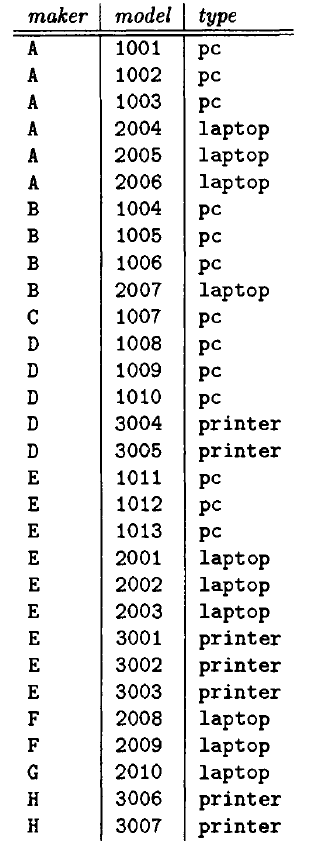
\includegraphics[width=0.4\textwidth]{hw3-1.png}
    \caption{Sample data for the relation \texttt{Product}.}
    \label{fig:sample-data-product}
\end{figure}

\begin{figure}[htbp]
    \centering
    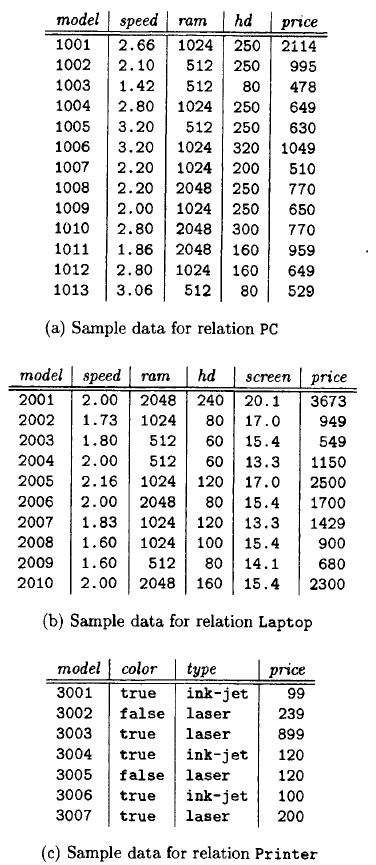
\includegraphics[width=0.4\textwidth]{hw3-2.png}
    \caption{Sample data for the relations \texttt{PC}, \texttt{Laptop}, and \texttt{Printer}.}
    \label{fig:sample-data-other}
\end{figure}

\begin{enumerate}
    \item[(a)] What PC models have a speed of at least 3.00?
    \item[(b)] Which manufacturers make laptops with a hard disk of at least 100GB?
    \item[(c)] Find the model number and price of all products (of any type) made by
          manufacturer B.
    \item[(d)] Find the model numbers of all color laser printers.
    \item[(e)] Find those manufacturers that sell Laptops, but not PC's.
    \item[(f)] Find those hard-disk sizes that occur in two or more PC's.
\end{enumerate}


\subsection*{Solutions}

\subsubsection*{(a) What PC models have a speed of at least 3.00?}

\[
    \pi_{\text{model}}(\sigma_{\text{speed} \geq 3.00}(\text{PC}))
\]

\subsubsection*{(b) Which manufacturers make laptops with a hard disk of at least 100GB?}

\[
    \pi_{\text{maker}} ( \sigma_{\text{hd} \geq 100} (\text{Laptop}) \bowtie
    \text{Product} )
\]


\subsubsection*{(c) Find the model number and price of all products (of any type) made by manufacturer B.}

\begin{align*}
    \pi_{\text{model},\ \text{price}} \bigg( & \
    ( \sigma_{\text{maker} = 'B'} (\text{Product}) \bowtie \text{PC} )     \\
                                             & \ \cup\
    ( \sigma_{\text{maker} = 'B'} (\text{Product}) \bowtie \text{Laptop} ) \\
                                             & \ \cup\
    ( \sigma_{\text{maker} = 'B'} (\text{Product}) \bowtie \text{Printer} )
    \bigg)
\end{align*}



\subsubsection*{(d) Find the model numbers of all color laser printers.}

\[
    \pi_{\text{model}} ( \sigma_{\text{color AND type='laser'}} (\text{Printer}) )
\]

\subsubsection*{(e) Find those manufacturers that sell Laptops, but not PC's.}

\[
    \pi_{\text{maker}} ( \sigma_{\text{type} = 'laptop'} (\text{Product}) )
    \ -\
    \pi_{\text{maker}} ( \sigma_{\text{type} = 'pc'} (\text{Product}) )
\]


\subsubsection*{(f) Find those hard-disk sizes that occur in two or more PC's.}
% SELECT hd FROM PC GROUP BY hd HAVING COUNT(*)>=2;
\[
    \pi_{\text{hd}} ( \sigma_{\text{COUNT}(\text{hd}) \geq 2} (\text{PC}) )
\]

\section{Exercise 2.4.3}

This exercise builds upon Exercise 2.3.2 concerning World War II capital ships. Recall it involves the following relations:

\begin{itemize}
    \item \texttt{Classes(class, type, country, numGuns, bore, displacement)}
    \item \texttt{Ships(name, class, launched)}
    \item \texttt{Battles(name, date)}
    \item \texttt{Outcomes(ship, battle, result)}
\end{itemize}

Figures \ref{fig:sample-data-table1} and \ref{fig:sample-data-table2} give some sample data for these four relations. Note that, unlike the data for Exercise 2.4.1, there are some ``dangling tuples" in this data, e.g., ships mentioned in \texttt{Outcomes} that are not mentioned in \texttt{Ships}.

Write expressions of relational algebra to answer the following queries. You may use the linear notation of Section 2.4.13 if you wish. For the data of Figs. \ref{fig:sample-data-table1} and \ref{fig:sample-data-table2}, show the result of your query. However, your answer should work for arbitrary data, not just the data of these figures.
\begin{figure}[htbp]
    \centering
    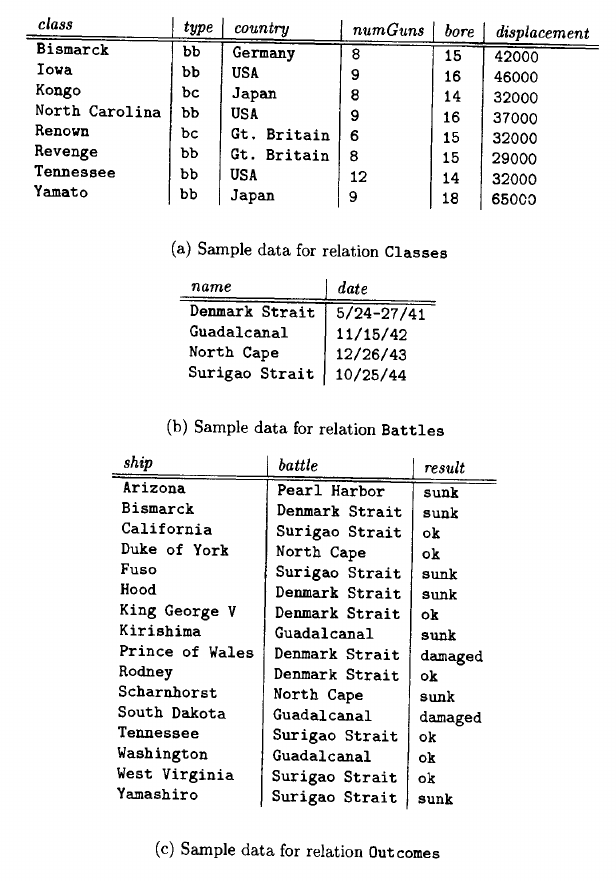
\includegraphics[width=0.8\textwidth]{hw3-3.png}
    \caption{Sample data for the relations \texttt{Classes}, \texttt{Ships}, \texttt{Battles}, and \texttt{Outcomes}.}
    \label{fig:sample-data-table1}
\end{figure}

\begin{figure}[htbp]
    \centering
    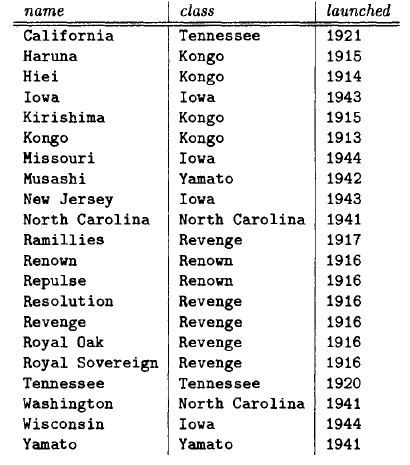
\includegraphics[width=0.6\textwidth]{hw3-4.png}
    \caption{Sample data for the relations \texttt{Ships} .}
    \label{fig:sample-data-table2}
\end{figure}

\begin{enumerate}
    \item[(a)] Give the class names and countries of the classes that carried guns of at least 16-inch bore.
    \item[(b)] Find the ships launched prior to 1921.
    \item[(c)] Find the ships sunk in the battle of the Denmark Strait.
    \item[(d)] The Treaty of Washington in 1921 prohibited capital ships heavier than 35,000 tons. List the ships that violated the Treaty of Washington.
    \item[(e)] List the name, displacement, and number of guns of the ships engaged in the battle of Guadalcanal.
    \item[(f)] List all the capital ships mentioned in the database. (Remember that all these ships may not appear in the \texttt{Ships} relation.)
\end{enumerate}



\subsection*{Solutions}

\subsubsection*{(a) Give the class names and countries of the classes that carried guns of at least 16-inch bore.}

\[
    \pi_{\text{class},\ \text{country}} ( \sigma_{\text{bore} \geq 16} (\text{Classes}) )
\]

\subsubsection*{(b) Find the ships launched prior to 1921.}

\[
    \pi_{\text{name}} ( \sigma_{\text{launched} < 1921} (\text{Ships}) )
\]

\subsubsection*{(c) Find the ships sunk in the battle of the Denmark Strait.}

\[
    \pi_{\text{ship}} ( \sigma_{\text{battle} = '\text{Denmark Strait}'} (\text{Outcomes}) )
\]

\subsubsection*{(d) The Treaty of Washington in 1921 prohibited capital ships heavier than 35,000 tons. List the ships that violated the Treaty of Washington.}

\[
    \pi_{\text{name}} ( \sigma_{\text{displacement} > 35000} (\text{Ships} \bowtie \text{Classes}) )
\]

\subsubsection*{(e) List the name, displacement, and number of guns of the ships engaged in the battle of Guadalcanal.}

\[
    \pi_{\text{name},\ \text{displacement},\ \text{numGuns}} (
    \sigma_{\text{battle} = '\text{Guadalcanal}'} (\text{Outcomes} \bowtie \text{Ships} \bowtie \text{Classes})
    )
\]

\subsubsection*{(f) List all the capital ships mentioned in the database. (Remember that all these ships may not appear in the \texttt{Ships} relation.)}

\[
    \pi_{\text{name}} ( \text{Ships} )
    \cup
    \rho_{S(\text{name})}(\pi_{\text{ship}} ( \text{Outcomes} ))
\]

\section{Exercise 2.5.1}

Express the following constraints about the relations of Exercise 2.3.1, reproduced here:

\begin{itemize}
    \item \texttt{Product(maker, model, type)}
    \item \texttt{PC(model, speed, ram, hd, price)}
    \item \texttt{Laptop(model, speed, ram, hd, screen, price)}
    \item \texttt{Printer(model, color, type, price)}
\end{itemize}


You may write your constraints either as containments or by equating an expression to the empty set. For the data of Exercise 2.4.1, indicate any violations to your constraints:

\begin{itemize}
    \item[(a)] A PC with a processor speed less than 2.00 must not sell for more than \$500

    \item[(b)] A laptop with a screen size less than 15.4 inches must have at least a 100 gigabyte hard disk or sell for less than \$1000

    \item[(c)] No manufacturer of PCs may also make laptops

    \item[(d)] A manufacturer of a PC must also make a laptop with at least as great a processor speed

    \item[(e)] If a laptop has a larger main memory than a PC, then the laptop must also have a higher price than the PC
\end{itemize}

\subsection*{Solutions}

\subsubsection*{(a) A PC with a processor speed less than 2.00 must not sell for more than \$500}

\[
    \sigma_{speed < 2.00 \ \mathbf{AND} \ price > 500} = \emptyset
\]

\subsubsection*{(b) A laptop with a screen size less than 15.4 inches must have at least a 100 gigabyte hard disk or sell for less than \$1000}

\[
    \sigma_{screen < 15.4 \ \mathbf{AND} \ hd < 100 \ \mathbf{AND} price \geq 1000}(Laptop) = \emptyset
\]

\subsubsection*{(c) No manufacturer of PCs may also make laptops}

\[
    \pi_{maker}(\sigma_{type=pc}(Product))\cap \pi_{maker}(\sigma_{type=laptop}(Product)) = \emptyset
\]

\subsubsection*{(d) A manufacturer of a PC must also make a laptop with at least as great a processor speed}

\begin{align*}
    R1 & := \pi_{maker, model, speed}(Product \bowtie PC)              \\
    R2 & := \pi_{maker, speed}(Product \bowtie Laptop)                 \\
    R3 & := \pi_{model}(R1 \bowtie_{R1.maker=R2.maker \ \mathbf{AND} \
    R1.speed > R2.speed} R2)                                           \\
    R4 & := \pi_{model}(R3) = \emptyset
\end{align*}

\subsubsection*{(e) If a laptop has a larger main memory than a PC, then the laptop must also have a higher price than the PC}
\begin{align*}
    R1 & := \pi_{ram, price}(PC)     \\
    R2 & := \pi_{ram, price}(Laptop) \\
\end{align*}

And we can get constraints such that

$$
    R1 \bowtie_{R2.ram > R1.ram \ \mathbf{AND} \
        R2.price \leq R1.price} R2 = \emptyset
$$

\section{Exercise 2.5.2}

Express the following constraints in relational algebra. The constraints are based on the relations of Exercise 2.3.2, reproduced here:

\begin{itemize}
    \item \texttt{Classes(class, type, country, numGuns, bore, displacement)}
    \item \texttt{Ships(name, class, launched)}
    \item \texttt{Battles(name, date)}
    \item \texttt{Outcomes(ship, battle, result)}
\end{itemize}

You may write your constraints either as containments or by equating an expression to the empty set. For the data of Exercise 2.4.3, indicate any violations to your constraints:

\begin{itemize}
    \item[(a)] No class of ships may have guns with larger than 16-inch bore.

    \item[(b)] If a class of ships has more than 9 guns, then their bore must be no larger than 14 inches.

    \item[(c)] No class may have more than 2 ships.

    \item[(d)] No country may have both battleships and battlecruisers.

    \item[(e)] No ship with more than 9 guns may be in a battle with a ship having fewer than 9 guns that was sunk.
\end{itemize}


\subsection*{Solutions}

\subsubsection*{(a) No class of ships may have guns with larger than 16-inch bore.}

\[
    \pi_{Class}(\sigma_{bore > 16}(Classes))= \emptyset
\]

\subsubsection*{(b) If a class of ships has more than 9 guns, then their bore must be no larger than 14 inches.}

\[
    \pi_{Class}(\sigma_{bore > 16\ \mathbf{AND} \ numGuns > 9}(Classes))= \emptyset
\]

\subsubsection*{(c) No class may have more than 2 ships.}

\begin{align*}
    R_1 & = \pi_{class, \text{COUNT}(name)}(ship) \\
    R_2 & = \sigma_{\text{COUNT}(name) > 2}(R_1)  \\
    R_2 & = \emptyset
\end{align*}

\subsubsection*{(d) No country may have both battleships and battlecruisers.}

\[
    \pi_{country}(\sigma_{type=battlecruiser}(Classes))\cap \pi_{country}(\sigma_{type=battleship}(Classes))= \emptyset
\]

\subsubsection*{(e) No ship with more than 9 guns may be in a battle with a ship having fewer than 9 guns that was sunk.}
    
\begin{align*}
    R1 & := \sigma_{numGuns > 9}(Classes)      \\
    R2 & := \sigma_{numGuns < 9}(Classes)      \\
    R3 & := (R1 \bowtie Ships) \bowtie Battles \\
    R4 & := (R2 \bowtie Ships) \bowtie
    \sigma_{result=sunk}(Battles)              \\
    R5 & := \pi_{battlename}(R3) \bowtie
    \pi_{battlename}(R4) = \emptyset
\end{align*}


\end{document}